\documentclass[times, utf8, diplomski]{fer}
\usepackage{booktabs}

\newcommand{\bplus}{B\textsuperscript{+}}
\newcommand{\rstar}{R\textsuperscript{*}}

\usepackage{graphicx}
\graphicspath{ {images/} }

\begin{document}

% TODO: Navedite broj rada.
\thesisnumber{000}

% TODO: Navedite naslov rada.
\title{System for tracking vehicle locations in real time}

% TODO: Navedite vaše ime i prezime.
\author{Arthur Dent}

\maketitle

% Ispis stranice s napomenom o umetanju izvornika rada. Uklonite naredbu \izvornik ako želite izbaciti tu stranicu.
\izvornik

% Dodavanje zahvale ili prazne stranice. Ako ne želite dodati zahvalu, naredbu ostavite radi prazne stranice.
\zahvala{}

\tableofcontents















% --------------INTRODUCTION-------------------------------------------------------------------------------------------------
\chapter{Introduction}
Vehicle location is a multidimensional data point, it can contain up to three dimensions of spatial data and even one dimension of temporal data. Dataset is comprised of many data points and can be either static or live -- in terms of supporting updates of vehicle locations. Of course, data is not worth anything if it can't be queried. Some common queries can be: what points are contained in given rectangle, or even more general in an arbitrary polygon. A query can be ask what points are contained within certain radius of a given point, but then another question arises -- how is distance defined in this space. A natural assumption is that the points are on planet Earth, but even Earth can be modelled in many ways, as a perfect sphere or as an ellipsoid, each one suitable for a different application in life. If temporal dimension is present then all of these queries can be appended with time interval to return only the points that are happened within that time.

% Another possibility is to add information about road positions and then try to match each vehicle to the closest point on the road. This means that a polygon query could be done in 

\section{Motivation}
Spatial and spatio-temporal data sets are growing rapidly. Consider these spatio-temporal data sets: Facebook or Foursquare with their check-ins, or photos on Instagram. These are all live datasets because queries and updates happen concurrently. There are also examples of static data sets such as data collected by Telecom providers -- a data point for each time a user's phone contacted the tower. This dataset is not live and could be used to perform analytics, usually in a MapReduce system, which has much different requirements on the design of the system.

Initial inspiration for the problem is Uber and similar applications. They have a large number of vehicles that update their location every few seconds. Each user's phone shows vehicles that are in a relatively small area of the map which gives a pretty clear picture of what the most relevant queries could be. Note that this is not a spatio-temporal dataset because only the last location of a vehicle is important, although one could easily imagine the version where the history of locations is stored and queried.

\section{Problem definition and constraints}
Let us define the problem more precisely. Each vehicle has a unique vehicle id and location. Location is encoded in a standard geographic coordinate system, as longitude and latitude pairs. Longitude is in [-180, 180] range and latitude [-90, 90].

Updating a location can be referred as \emph{update $(vehicle\_id, longitude, latitude$)}.

The simplest possible query is to find a list of vehicles that are within a given rectangle, and is referred as
$$rectangle\_query (longitude\_min, longitude\_max, latitude\_min, latitude\_max)$$
A point with its longitude and latitude is inside a given rectangle iff $longitude\_min <= longitude <= longitude\_max$ and $latitude\_min <= latitude <= latitude\_max$.

Another interesting query is to search for points within certain distance of a given point.  Let's refer to this query as
$$radius\_query (longitude, latitude, radius)$$

Notice that the rectangle query was defined in a general way, it could be applied to any two dimensional data set, but this query needs a definition of distance between two points. We will use the simplest Earth model, a perfect sphere with quadratic mean radius of 6372 km. This choice is acceptable because distances should be fairly small and precise geometrical calculations are not mission critical. In turn, this should make geometry calculations as simple and as fast as possible.

Number of vehicles and users in this system is not defined in advance but is expected to be large so the requirement is that the system shouldn't be constrained by only one computer, i.e. must be scalable. Persistency of the data is not important because all of the data is only relevant for a short period of time, which isn't good enough reason to further complicate the system with persistence considerations. Also, if persistence is needed it can be achieved by another system which can be developed independently from this one and will not be studied in this thesis. 

Consistency - eventual - not 100\% sure?

\chapter{Background}
Historically, relational databases (RDBMs) have been the most popular storage system, and still are today. Geographical data and the need to store and query it has also been present in computer science for a long time. This is why most of the solutions were developed on top of relational RDBMS. The most important indexing data structure in RDBMs are B- and \bplus-trees and they work very well with one dimensional data. Those trees then formed the basis of R- and \rstar-trees which became the standard for spatial queries in RDBMs because this design enabled great interoperability with existing RDBMs.

RDBMs have trouble in keeping up with the massive data growth in recent years mainly because of its scalability issues. This is why there has been a rise of NoSql databases that are designed to scale much better. This of course comes with a cost of supporting only a fraction of features that RDBMs support and often lack the same consistency guarantees. To improve on those basic scalability issues it is necessary to completely move from RDBMs to distributed storage systems even though that means that classical approaches such as \rstar-trees won't work.

\section{Traditional solutions}
Lets make a step back and briefly describe the traditional solutions in RDBMS -- R-tree \cite{rtree} and its improvement \rstar-tree \cite{rstar}.

R-tree is a height-balanced tree similar to a B-tree with every node except root containing between $m$ and $M$ records. $M$ is chosen to store the largest possible number of records before it grows to big to fit inside a single disk page. Every record contains information about minimal bounding box $I$ it is "responsible" for. This means that all the data in its subtree is within this bounding rectangle $I$, but that doesn't mean that some other node doesn't contain any points from this area. Bounding box can be represented as $I = (I_x, I_y)$ where $I_x$ and $I_y$ are intervals $[a, b]$ defining what interval on $x$ and $y$ axes current record contains. Records in non-leaf nodes contain minimal bounding box of its subtree. Leaf nodes contain pointers to actual geometrical objects stored, but minimal bounding box is also computed and stored in them.

The most basic search query is to search for points within a given rectangle $R$. Search starts from the root node and recursively traverses the tree but only to nodes whose bounding box $B$ intersects with $R$. If $R$ completely contains $B$ than whole subtree should be returned, otherwise search continues in all of the children nodes.

Inserting a new point is similar to search. New record is always inserted in the leaf node. If a node gets too big it has to be split and splits propagate up the tree. There are many heuristics on how to choose the appropriate leaf node to insert a new record. R-tree, at each level, always chooses the node which needs the least enlargement to fit a new point. Splitting a node also employs heuristics because there are $2^M-1$ combinations to split it.

\rstar-tree improves on the R-tree by introducing better heuristics to split a node and to find the best node when inserting a new point.

Estimating the complexity of inserting and search isn't easy, but the main idea is that the search algorithm on average won't need to retrieve many data points that are not inside the query box.

\section{Geohash}
Geohashing is a method of transforming two dimensional data into one dimension such that the points that are close in the original space are usually close in the transformed space.

Input to the geohash function is a point on the map and the output is a bit string of arbitrary length -- greater length means greater precision. Construction works by repeatedly splitting the input space in half and output a $0$ if in left half and $1$ otherwise, in each step alternating between splitting vertically or horizontally.

Let's give an example of how to encode a point in Beijing $116^{\circ}23'$ E $39^{\circ}55'$ N. It is easier to work with if converted to more appropriate form $(116.38, 39.92)$. 

\begin{center}
\begin{tabular}{ |c|l|l|l| } 
	\hline
	Precision & Longitude range & Latitude range & Geohash \\
	\hline
	0 & $[-180, 180]$ & $[-90, 90]$ & -- \\ 
	1 & $[0, 180]$ & $[-90, 90]$ & 1 \\ 
	2 & $[0, 180]$ & $[0, 90]$ & 11 \\ 
	3 & $[90, 180]$ & $[0, 90]$ & 111 \\ 
	4 & $[90, 180]$ & $[0, 45]$ & 1110 \\ 
	5 & $[90, 135]$ & $[0, 45]$ & 11100 \\ 
	6 & $[90, 135]$ & $[22.5, 45]$ & 111001 \\ 
	7 & $[112.5, 135]$ & $[22.5, 45]$ & 1110011 \\ 
	8 & $[112.5, 135]$ & $[33.75, 45]$ & 11100111 \\ 
	9 & $[112.5, 123.75]$ & $[33.75, 45]$ & 111001110 \\ 
	10 & $[112.5, 123.75]$ & $[39.375, 45]$ & 1110011101 \\ 
	11 & $[112.5, 118.125]$ & $[39.375, 45]$ & 11100111010 \\ 
	12 & $[112.5, 118.125]$ & $[39.375, 42.1875]$ & 111001110100 \\ 
	13 & $[115.3125, 118.125]$ & $[39.375, 42.1875]$ & 1110011101001 \\ 
	14 & $[115.3125, 118.125]$ & $[39.375, 40.78125]$ & 11100111010010 \\ 
	\hline
\end{tabular}
\end{center}

The first column shows longitude range that the current geohash represents and the second column shows the same thing for latitude. The process starts by splitting the longitude range in half and since the point has longitude larger than zero, bit 1 is appended. In the next step the same happens for latitude, and then the algorithm continues to alternate between splitting longitude and latitude ranges. The odd indexed bits are result of splitting by longitude, and even indexed bits are result of splitting by latitude. With every added bit of precision one of the range's size splits in half, which means that geohash always represents a rectangle.

It is now pretty obvious that two geohashes which have a common prefix $P$ are within the rectangle that is represented by that prefix $P$. This is why we say that geohashing preserves \emph{locality}. Note, that if two points are close, it doesn't mean that they will have a common prefix at all. For example, two points that are very close to each other, but are at the different sides of the prime meridian will have a different first bit, and therefore no prefix in common. This is something that needs to be paid attention at when designing geohash algorithms.

\begin{figure}[h]
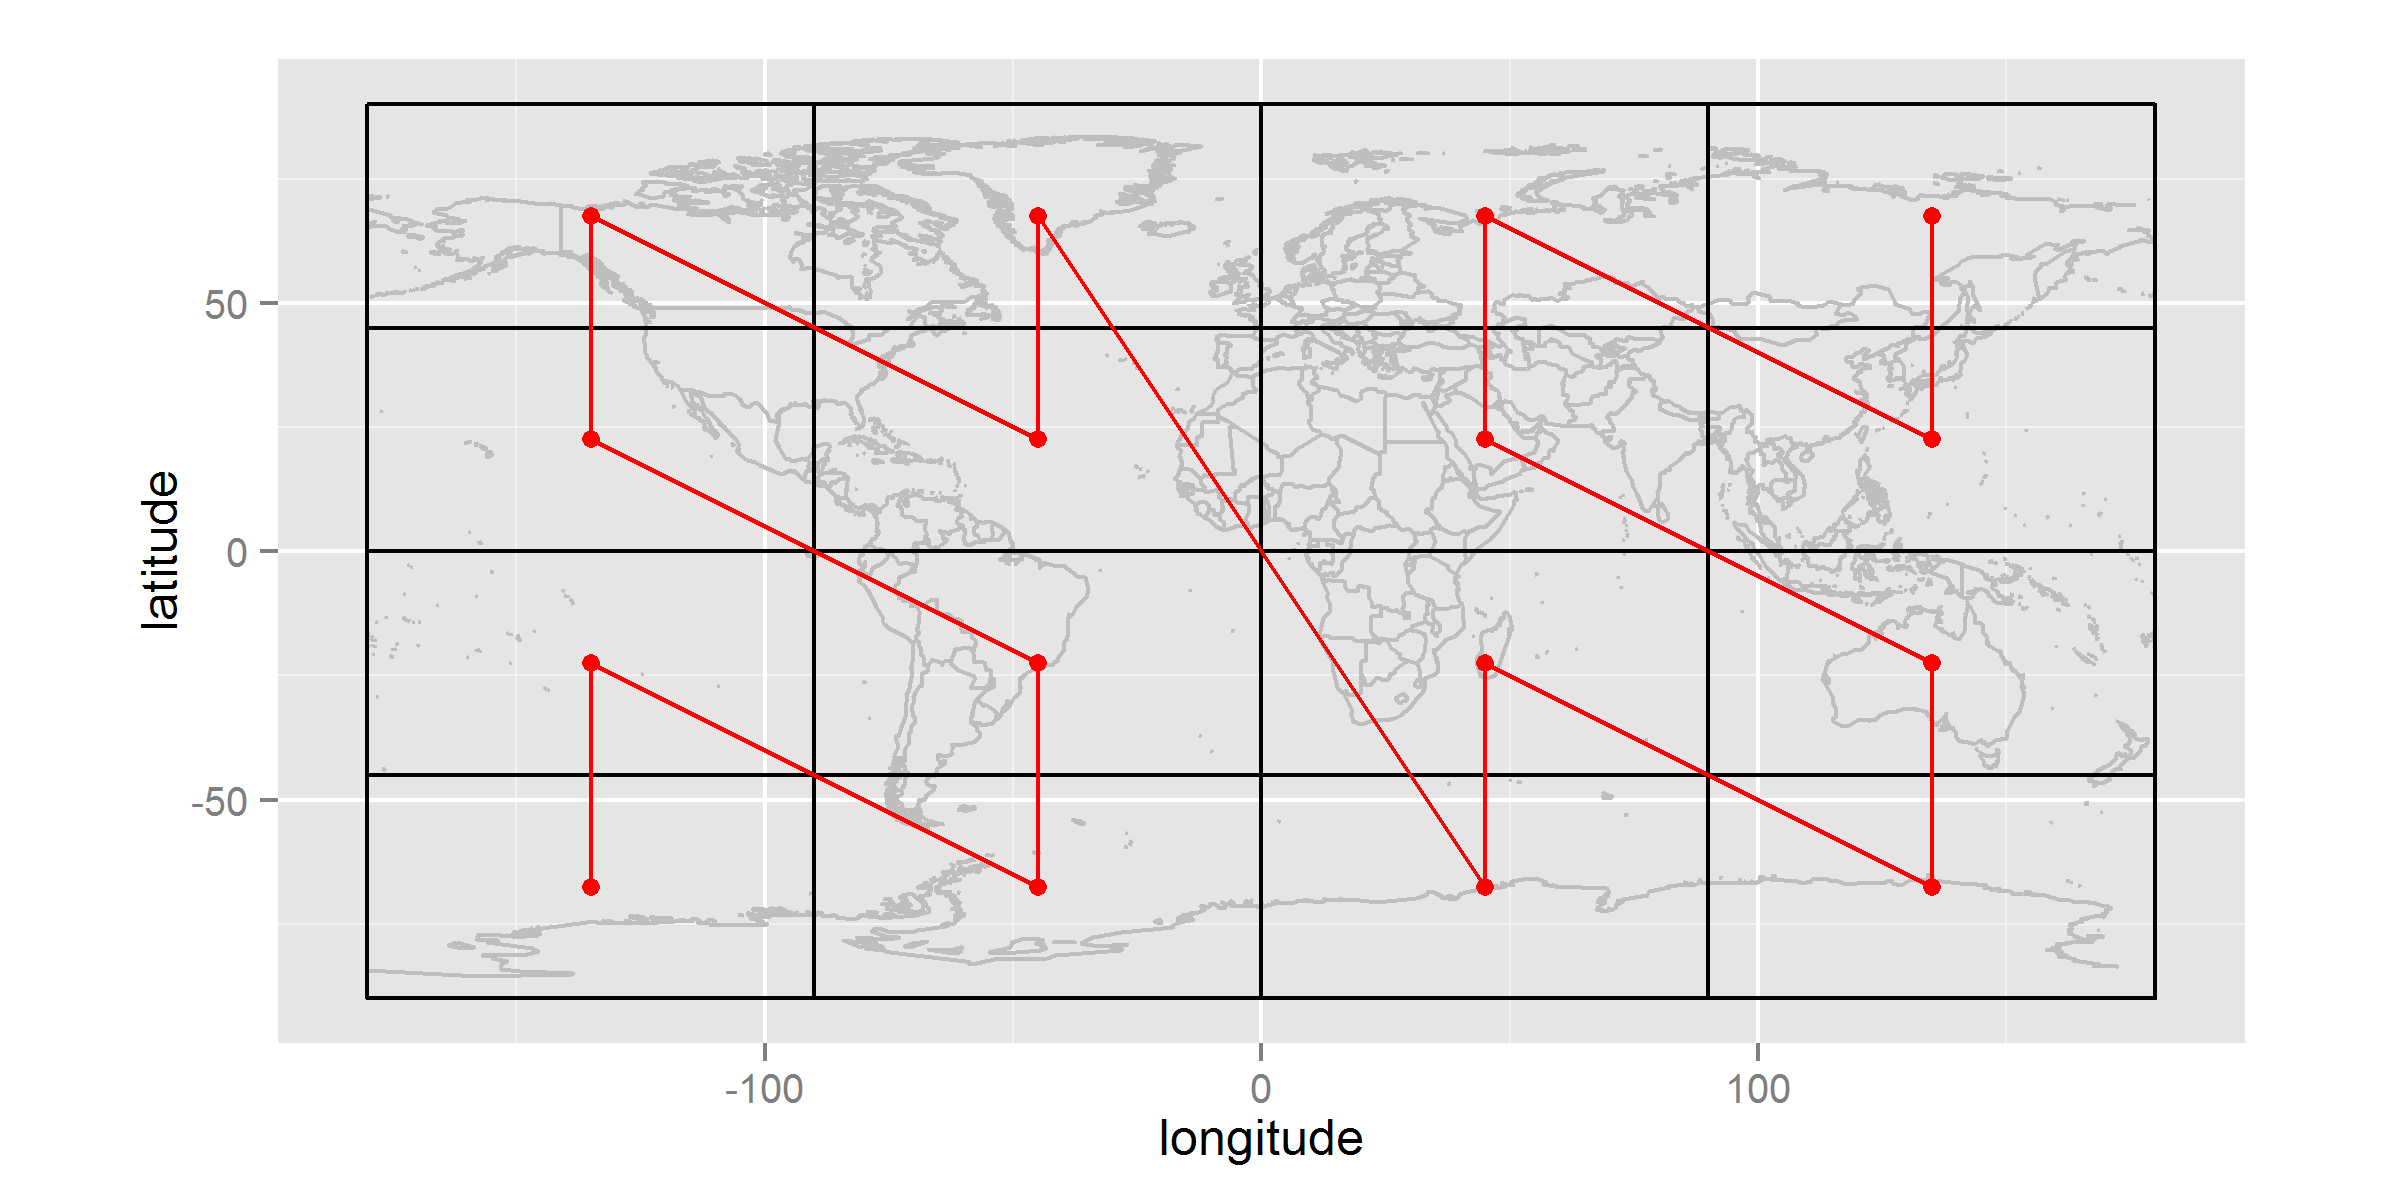
\includegraphics[width=\textwidth]{z_curve}
\caption{Z-order curve with precision 4 \cite {spatiotemporal}}
\label{fig:zcurve}
\end{figure}

Figure \ref{fig:zcurve} shows all geohashes with precision 4, sorted and plotted with lines drawn between neighbouring elements. It is a mathematical object called z-order curve \cite{zcurve} and it appears at any chosen precision.

In order to be able to answer a rectangle query it is necessary to have an algorithm that can find geohashes that cover an arbitrary rectangle completely. This is known as a rectangle coverage problem. One goal is to use as few geohashes as possible and the other goal is to "over cover" the smallest possible area. If the second goal didn't exist, the solution would always be to use an empty geohash because it covers every rectangle. If we wanted to perfectly cover the rectangle, it might happen that infinite number of geohashes is required. The following simple algorithm will provide a solution with respect to both goals.

The idea is to find a central geohash -- one that covers the center point of the rectangle, and then find all 8 neighbouring geohashes and return them with the central geohash. All of those geohashes will have the same precision. All that is left is to find the largest precision that guarantees that the whole rectangle gets covered. The condition in one dimension, e.g. longitude, at certain precision level is that $2*W >= L$ where $W$ is length of longitude side of rectangle and $L$ length of geohash longitude range. If that condition holds it means that the central geohash and it's left and right neighbour cover this longitude range. When constructing the central geohash, with each added bit, this condition must be checked. If it doesn't hold, than the last bit must be removed and the algorithm stops.

This approach returns 9 geohashes, but it might happen that not all of them even intersect the original rectangle, so those can be omitted. It turns out if the returned geohashes are sorted, then many of the neighbouring elements will differ only by one. This start to make sense if you take a look at Figure \ref{fig:zcurve} where you can see how the consecutive geohashes are ordered on the map -- very often two consecutive geohashes are neighbours in one of the 8 directions which is also the pattern of the returned geohashes. Instead of returning a list of geohashes, we can return a list of geohash ranges that cover the rectangle. Empirically, this resulting list of ranges usually has two or three elements which is much better than 9 elements in the original list.

\section{Key-value stores}
Key-value stores are non relational databases.
As mentioned before geohashes provide a way to map two dimensional data into one dimension while preserving locality. It was also showed how to cover a rectangle with only few geohash ranges. This means that the system has to be able to retrieve all geohashes from a certain range. If all geohashes are stored in a sorted set, it is possible to find the first element from the range and iterate until the end of the range. As mentioned, rectangle coverage usually covers more area than requested, which means that when each element is returned from the set it has to be checked wether it really is within the rectangle.

This is where distributed key-value stores come to play. The criteria is that this data store is able to store keys in some sort of a sorted manner. One of the initial requests is that persistence is optional, and real time performance is more important. That's why a \emph{distributed in-memory database} is the best solution.

In few other relevant papers where they built spatial \cite{spatialindex} and spatio-temporal \cite{spatiotemporal} distributed indexes, they used HBase and Accumulo both based on Google's BigTable implementation. We didn't go with that choice because those are not in-memory databases.

We chose \emph{Redis} which is an in-memory key-value store with support for many different data types, and one of them is an ordered set called \emph{ZSET}. Originally Redis wasn't a distributed database, but in the past few years Redis Cluster was developed. Redis Cluster shards the data based on its key, but it can not shard within a single key which is needed because we would like to store all the geohashes inside a single key of type ZSET. This means that we will have to handle this part manually, by creating multiple ZSET keys and querying the appropriate ones.

ZSET orders elements by their score, which is a 64-bit floating point number that can store integer values without the loss of precision, only if value is in range $[-2^{53}, 2^{53}]$. This score will be used to store geohash values with \emph{52 bit precision}. Those 52 bits are more than enough -- latitude resolution with 26 bits is $180^{\circ}/2^{26} \approx 2.6^{\circ}*10^{-6}$, or about 10 cm. Along with score, each element can store a string value called \emph{member}. It will be used to store a vehicle id.

% Deliberately not explaining GET/SET.

The main question is how to shard the sorted set and be able to do updates and answer rectangle queries efficiently. The next two chapters will describe the two approaches that were implemented.


\chapter {Prefix sharding}
One way to distribute keys is to create more keys then the number of nodes and hope that approximately the same number of keys ends up on each node. Just as geohashing preserves locality, it is useful to try to do the same when designing the sharding scheme. This is achieved by sharding based on geohash prefix. When a point is added to the system, geohash is computed and it is inserted into one of the sorted sets based on its first $P$ bits. Each set is named based on the prefix it represents and all of the points inside that set share the same prefix. $P$ is an adjustable parameter that can be tuned based on the expected data set. Each prefix set is created lazily -- only when a point with such prefix is inserted.

As already said, rectangle query boils down to answering what points are in a geohash range. It is possible that a requested geohash range spans through multiple prefix sets, so a range might be split in multiple ranges such that each of them contains only geohashes with the same prefix. This is an unlikely event if queried rectangles are significantly smaller than the area represented by geohash of precision $P$.

Obvious advantage with this approach is that the rectangle query is very fast, and in most cases it doesn't make any more requests to Redis than the non-distributed variant. Insertion is also simple, just an appropriate prefix set has to be chosen and inserted to.

Downside is that $P$ has to be chosen in advance. If it has to be changed later, all points need to be reinserted. A bit more subtle performance issue is that it is sensitive to spatial distribution of queries. If a small area on the map becomes hot, all the requests will fall into a small number of prefixes and only a fraction of nodes will be utilised.

% What about updates?

\chapter {Vehicle id sharding}

\chapter {Design and implementation}
\section {Redis geo features}
\section {Experimental setup}
\section {Test data}

\chapter {Results}

\chapter{Conclusion}
Conclusion.

\bibliography{literatura}
\bibliographystyle{fer}

















% ----------------------------------Summary------------------------------------------------------
\begin{sazetak}
Sažetak na hrvatskom jeziku.

\kljucnerijeci{Ključne riječi, odvojene zarezima.}
\end{sazetak}

% TODO: Navedite naslov na engleskom jeziku.
\engtitle{Title}
\begin{abstract}
Abstract.

\keywords{Keywords.}
\end{abstract}

\end{document}
